\documentclass[conference]{IEEEtran}
\IEEEoverridecommandlockouts
% The preceding line is only needed to identify funding in the first footnote. If that is unneeded, please comment it out.
\usepackage{cite}
%\usepackage[toc,page]{appendix}
\usepackage{amsmath,amssymb,amsfonts}
\usepackage{algorithmic}
\usepackage{graphicx}
\usepackage{textcomp}
\usepackage{xcolor}
\usepackage{listings}
\lstset{
  basicstyle=\ttfamily,
  columns=fullflexible,
  frame=single,
  language=Python,
  breaklines=true,
%  postbreak=\mbox{\textcolor{red}{$\hookrightarrow$}\space},
}
\def\BibTeX{{\rm B\kern-.05em{\sc i\kern-.025em b}\kern-.08em
    T\kern-.1667em\lower.7ex\hbox{E}\kern-.125emX}}
\begin{document}

\title{Project 11: Semantic Analysis 1}

\author{\IEEEauthorblockN{Dennis Neumann}
\IEEEauthorblockA{Oulu, Finland\\
dennis2.neumann@student.uni-siegen.de}
\and
\IEEEauthorblockN{Muhammad Sheraz Khan}
\IEEEauthorblockA{Oulu, Finland\\
Sherazkhan1234@gmail.com}
}

\maketitle
\begin{abstract}
Semantic similarity has been used for multiple tasks regarding natural language processing for many years now. Various static and lexica-based methods for analyzing semantic similarity such as Wu-Palmer and Leacock-Chodorow with different approaches and results exist to determine the similarity between given phrases. This project aims to show how dynamic and web-based similarity methods work in comparison to the static methods with the help of the Python Natural Language Toolkit and Google Search API.
\end{abstract}

\begin{IEEEkeywords}
semantic similarity, natural language processing, language processing, semantic, analysis, google search
\end{IEEEkeywords}

\section{Introduction}

Over many decades, for many tasks regarding semantic similarity there have been methods introduced. Based on the proposal of Rada et. al. \cite{rada89}, similarity of synonym sets (synsets) describes the minimum distance from one node to another in a taxonomical tree. Since this approach assumes, that the links in the taxonomy represent uniform distances \cite{resnik} between two words, some approaches derive their own measurement methods which try to solve this problem. Wu-Palmer similarity (WUP) \cite{wupalmer}, Path similarity (PATH) \cite{resnik} and Leacock-Chodorow Similarity (LCH) \cite{lch} proposed their own approaches and use the English database WordNet, which groups English words into synonym sets (synsets) according to similar meanings and lexical relations \cite{wordnet}. WUP considers the depth in two synsets, as concepts of words become more similar the lower they lie in the ontological hypernim tree \cite{wupmod}. PATH calculates the shortest distance between the synsets, but other than the solution of Rada et. al, it considers the fact, that some sub-trees of a taxonomy are deeper than others \cite{resnik}. LCH calculates the overall shortest path between two given concepts \cite{slimani} to their common hypernyms in the taxonomy tree \cite{perkins}.\\
However, those are static methods and only work on formal words, not considering slang or buzzwords. Moreover, meanings of words or relations to such can change over time \cite{websim}, for example the word \textit{Tesla} nowadays can not only be associated with Nikola Tesla but also with the electric car brand of the same name. Therefore, this project aims to show some dynamic approaches like the WebJaccard similarity (WebSim). Those are based on web search engines and try to determine the correlation between the given words or phrases according to the web search results.\\
Chapter~\ref{sec:methodology} introduces to the used tools and libraries. Chapter~\ref{sec:implementation} shows the implementation details. In chapter~\ref{sec:results} the achieved results are shown and discussed.  Chapter~\ref{sec:results} concludes this project documentation and sums up the content.

\section{Methodology}\label{sec:methodology}

\subsection{Word pairs}

According to the requirements for this project, the similarity methods have to be applied on at least ten synonym sets pairs \textit{(P,Q)}. The pairs should include the three cases, in which a) \textit{P} is a synonym of \textit{Q}, b) \textit{P} is an antonym of \textit{Q}, c) \textit{P} has an entailment relation to \textit{Q}. For the tasks of this project, following word pairs were selected:
\begin{itemize}
\item pleased - excited
\item run - rush
\item displeased - upset
\item sleep - nap
\item laugh - weep
\item rich - poor
\item drunk - sober
\item mobile phones - cell phones
\item introvert - extrovert
\item huawei - iphone
\item run - sweat
\item contested - won
\item fell - broken
\end{itemize}
Many synsets are not applicable to use together in some of the similarity methods, since they are not sharing common hypernyms \cite{perkins}. Therefore, the choice of word pairs is very important for applying and testing them against all similarities. This issue is discussed further in chapter~\ref{subsec:wup}.

\subsection{Tools and Libraries}
\begin{itemize}
\item \textbf{Natural Language Toolkit (NLTK)}: For overall processing human language words
\item \textbf{Google Search API} and \textbf{Custom Search API}: For later discussed websearch-based similarity methods
\item \textbf{Levenshtein}: Python package for calculation of Levenshtein distance
\item \textbf{re}: Regular expression package to process regular expressions
\item \textbf{Matplotlib}: Calculate data relations
\item \textbf{Seaborn}: Visualization of calculated data relations
\item \textbf{Pandas}: For implementation of tables
\item \textbf{Tkinter}: Python Interface programming
\end{itemize}

\section{Implementation}\label{sec:implementation}

\subsection{Preliminary Work}

For the purposes of understanding and for avoiding recurring code segments, this short chapter shows code snippets related to the implementations in the following chapters.

\subsubsection{Gihub Repository}

The source code and this report are available in the following Github repository: https://github.com/dneumann20/NLPproject.

\subsubsection{Visualization of Synsets and Results}

To visualize the similarity results for the word pairs defined in chapter~\ref{sec:methodology}, the word pairs are saved to the table \textit{pair\_words\_df} via the \textit{DataFrame} Python class. For every similarity, 

\begin{lstlisting}[frame=single, label=lst:table, caption={}, captionpos=b]]
sim_layer = [['pleased', 'Excited'], ['run', 'rush'], ...]
...
pair_words_df = pd.DataFrame(sim_layer, columns=['P', 'Q'])
pair_words_df['Column name'] = ''

for i in range(len(synsets)):
    pair_words_df.iloc[i,k] = ...
\end{lstlisting}

\subsubsection{Pre-Processing function}\label{sec:preproc}

In case of synsets of word length>1,  pre-processing should be performed. It has to contain the conversion in lower case, removal of special characters and lemmatizer for removing words with only one character as well as stopwords. The code snippet~\ref{lst:preproc} demonstrates the important steps taken for the pre-processing with the python package \textbf{re}.

\begin{lstlisting}[frame=single, label=lst:preproc, caption={Pre-processing for synsets of word length>1}, captionpos=b]]
def pre_processing(text):

    text = text.split(' ')
    text = [word.strip().lower() for word in text if word.lower() not in stopwords]
    rx = re.compile('([&#.:?!-()])*')
    text = [rx.sub('', word) for word in text]
    
# selecting only the alpha bets and words length greater than 1
    text = [word for word in text if len(word)>1 and word.isalpha()]
#     if some word appear more than 1, remove others
    unique = set(text)
    unique = [lemmatizer.lemmatize(word) for word in unique]
    
# storing after processing in third column
    return ' '.join(text)
\end{lstlisting}

\subsection{WebJaccard page count similarity}\label{subsec:webjac}

The first task consists of implementing the WebJaccard similarity based on page count and calculate the similarity coefficient. Where \textit{H(P)} in \ref{fig:pagecount} are the results of the pair key P and \textit{H(Q)} the results of pair key Q, \textit{H(PQ)} are the results when searching for P and Q together. This similarity coefficient  is calculated as followed in figure~\ref{fig:pagecount}:

\begin{figure}[h]
\centerline{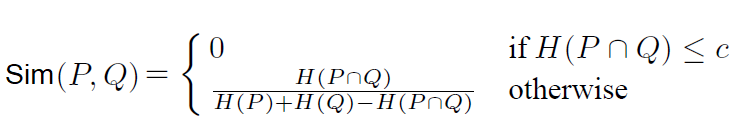
\includegraphics[scale=0.6]{img/pagecount.png}}
\caption{Formula for page-count-based WebJaccard similarity \cite{websim}.}
\label{fig:pagecount}
\end{figure}

For the implementation the Google Search API was used. For proper use of the \textit{search()} function, some parameters have to be considered as seen in~\ref{lst:googlesearch}: whereas \textit{num} is the number of results and the maximum number is 10, the maximum request number per day is 100. The \textit{pause} between every requests also needs to be adjusted as a too high amount might slow down the process too much and a too low number might end up in an IP block by Google \cite{search}.

\begin{lstlisting}[frame=single, label=lst:googlesearch, caption={Google search function}, captionpos=b]
def google_search(query):
    return search(query, lang = 'en', num = 10, start = 0, stop = None, pause = 2.0)
\end{lstlisting}

Now the function can be used to get the results for each pair (P,Q). To get the page count, the \textit{len()} function is used on the returned \textit{list} of results (see~\ref{lst:hpq}). Once each \textit{H(P)}, \textit{H(Q)} and \textit{H(PQ)} results are saved in according variables \textit{count\_p}, \textit{count\_q} and \textit{count\_pq}, they can be used to calculate the Jaccard similarity coefficient. The \textit{threshold} is used to determine the minimum number of results. If the number of results is less than the threshold, the coefficient is 0 \cite{websim}. For the chosen word pairs, there is no need for pre-processing the input since they only contain one word. Since the google API has a limitation of searching for one pair per hour, the values of the WebJaccard similarity had to be calculated one after another. To save the time, the calculated values were saved inthe array \textit{web\_results}.

\begin{lstlisting}[frame=single, label=lst:hpq, caption={Getting google results and calculation of WebJaccard similarity}, captionpos=b]]
def sim(P, Q, threshold, pre_process=False):
    if pre_process:
        P = pre_processing(P)
        Q = pre_processing(Q)

    results_p = google_search(P)
    count_p = len(list(results_p))

    results_q = google_search(Q)
    count_q = len(list(results_q))
    
    results_pq = google_search('{} AND {}'.format(P,Q))
    count_pq = len(list(results_pq))
    
    if count_pq <= threshold:
        return 0
    
    else:
        return (count_pq) /(count_p + count_q - count_pq)
...
web_results = [0.700, 0.960, 0.564, ...]
\end{lstlisting}

\subsection{Wu-Palmer-, Path- and Leacock-Chodorow-Similarity}\label{subsec:wup}

Unlike the WebJaccard similarity which has to be implemented manually, the WordNet Python library has predefined functions for WUP as well as PATH and LCH. This way, \textit{wup\_similarity()}, \textit{path\_similarity()} and \textit{lch\_similarity()} can be easily used on the self defined synsets from~\ref{sec:methodology}. The only pre-processing which has to be taken care of is to convert all synset's characters to lower case.\\
As seen in picture~\ref{fig:wupform}, WUP takes the depths of each synset as well as their least common subsumer (LCS) in account \cite{mohit}:

\begin{figure}[h]
\centerline{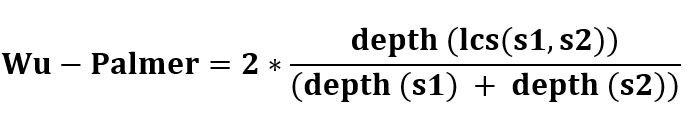
\includegraphics[scale=0.4]{img/wupalmer.jpg}}
\caption{Formula of WUP \cite{mohit}.}
\label{fig:wupform}
\end{figure}

LCH as a derived form of PATH is calculated as a negative log of shortest path (spath) of two phrases\cite{mohit}. The formula is described as followed in pciture~\ref{fig:lchform}:

\begin{figure}[h]
\centerline{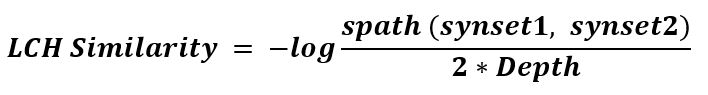
\includegraphics[scale=0.4]{img/lch.jpg}}
\caption{Formula of LCH \cite{mohit}.}
\label{fig:lchform}
\end{figure}

Code snippet~\ref{lst:wup} shows the use of the predefined similarity functions mentioned above.

\begin{lstlisting}[frame=single, label=lst:wup, caption={Use of WUP, PATH and LCH}, captionpos=b]
P.lch_similarity(Q)
P.wup_similarity(Q)
P.path_similarity(Q)
\end{lstlisting}

\subsection{Snippet Similarity}\label{subsec:wup}

For this task, the similarity between multiple snippets (SnippetSim)  from google search have to be calculated. To retrieve the results, Google's Custom Search JSON API was used. First an API key has to be created and a Custom Engine ID (\textit{cx}) generated (see code snippet~\ref{lst:snippetsim1}). These have to be inserted in the corresponding function \textit{build()} and class \textit{Customsearch.Cse.List} to make the source code work.

\begin{lstlisting}[frame=single, label=lst:snippetsim1, caption={Connection to Google Search API}, captionpos=b]
def google_snippets1(query, num=10):

    query_service = build(serviceName="customsearch", version="v1", developerKey='...')

    query_results = query_service.cse().list(q=query,cx='...', num=num).execute()
     return query_results['items']
\end{lstlisting}

For this similarity, the preprocessing function~\ref{lst:preproc} from chapter~\ref{sec:preproc} has to be used. For the calculation of the SnippetSim in this project, the first 5 results were taken. The implementation of the SnippetSim looks roughly as followed in~\ref{lst:snippetsim2}):

\begin{lstlisting}[frame=single, label=lst:snippetsim2, caption={Calculation of SnippetSim}, captionpos=b]
def sim_snippets1(p, q):
  for i in range(5):
        snippets_p += pre_processing(p)    
... 
        snippets_q += pre_processing(p)
...    
    common_words = len(set(snippets_p.strip().split(' ')) & set(snippets_q.strip().split(' '))) 
    combined_unique_words = len(set(snippets_p + snippets_q))
    
  return common_words/combined_unique_words
\end{lstlisting}

\subsection{Snippet Overlapping Similarity}\label{subsec:olsim}

Another similarity using snippets is based on overlapping percentage between two phrases. In this report, it will be shortened as OLSim. This task needs a special pre-processing technique called the Levenshtein distance \cite{levenshtein}, also called editing distance. It calculates the number of operations needed to change one phrase to another by changing one character after another. The allowed operations are insertions, deletions and substitutions \cite{navarro}. The formula of the Levenshtein distance is described as followed in picture~\ref{fig:lev}:

\begin{figure}[h]
\centerline{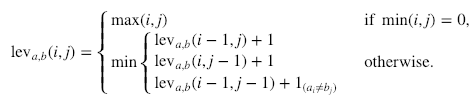
\includegraphics[scale=0.6]{img/lev.png}}
\caption{Formula for Levenshtein distance \cite{fuzzy}.}
\label{fig:lev}
\end{figure}

The first row corresponds to deletion, the second row to insertion and the third row to substitution \cite{fuzzy}. The Levenshtein ratio is the corresponding similarity ratio derived from the Levenshtein distance \cite{fuzzy} and is defined in picture~\ref{fig:levratio}:

\begin{figure}[h]
\centerline{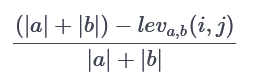
\includegraphics[scale=0.6]{img/levratio.png}}
\caption{Formula for Levenshtein similarity ratio \cite{fuzzy}.}
\label{fig:levratio}
\end{figure}

Similar to SnippetSim, the implementation of the OLSim is roughly as followed in code snippet~\ref{lst:olsim}:

\begin{lstlisting}[frame=single, label=lst:olsim, caption={Calculation of OLSim}, captionpos=b]
def sim_snippets2(p, q):
    for i in range(10):
...
        snippets_p += pre_processing(p)
...
        snippets_q += pre_processing(q)   
...
    return round(lev.ratio(snippets_p, snippets_q),4)
\end{lstlisting}

\subsection{Human Judgement Score}\label{subsec:humanjudge}

In this task, the human judgement score (HJS) according to Miller \& Charles (MC-28)  \cite{miller} was taken to calculate the correlation to the similarity methods from chapter~\ref{subsec:wup} by using the Pearson coefficient. Exceptionally for this case, the following five pairs from the openly available datasets MC-28 \cite{miller} were used:

\begin{itemize}
\item automobile - car
\item gem - jewel
\item journey - voyage
\item boy - lad
\item coast - shore
\end{itemize}

Similar to~\ref{lst:table}, a table is created in code snippet~\ref{lst:hjs} and the mentioned dataset is embedded.

\begin{lstlisting}[frame=single, label=lst:hjs, caption={HJS correlation with WUP, PATH, LCH}, captionpos=b]
df_mc = pd.read_csv('mc.csv', sep=';', names=['Word 1', 'Word 2', 'Human Judgement Score'])
df_rg = pd.read_csv('rg.csv', sep=';', names=['Word 1', 'Word 2', 'Human Judgement Score'])
df_wordsim = pd.read_csv('wordsim.csv', sep=';', names=['Word 1', 'Word 2', 'Human Judgement Score'])
...
data = pd.concat([df_mc, df_rg, df_wordsim])
data.head()
\end{lstlisting}

Although the final output shows the mentioned pairs earlier in this chapter, it also shows the way how other datasets like RG (Rubenstein and Goodenougth, 1965) or WordSim353 (Finkelstein et al., 2001) can be embedded as well.\\
To calculate and plot each correlation from the table created in the code above, the function in code snippet~\ref{lst:corr} was implemented. For the visualization, the \textit{scatter} plot was used and the \textit{despine} function for the removal of unnecessary axis. After that the correlation can be calculated with the \textit{corr()} function.

\begin{lstlisting}[frame=single, label=lst:corr, caption={Correlation calculation function}, captionpos=b]
import matplotlib.pyplot as plt
import seaborn as sns

def plotting_correlation(data, col1, col2):
    ...
    plt.scatter(data[col1], data[col2])
    sns.despine()
    corr = round(data[[col1, col2]].corr().iloc[0,1], 3)
   ...
    plt.show()
\end{lstlisting}

\subsection{Similarity GUI}\label{subsec:gui}

This project also includes a GUI to run all previously implemented similarity methods by clicking corresponding buttons. The source code for the GUI implementation included in the appendix chapter~\ref{sec:append}.

\section{Results and discussions}\label{sec:results}

\subsection{Results of web-based and lexica-based Solutions}

As mentioned in chapter~\ref{sec:methodology}, many pair words exist in which the combination of such do not work together, which causes some of the methods showing the similarity results as "None" \cite{perkins}, or in the case of LCH the pairs cause a compilation error "Computing the lch similarity requires synset1 and synset2 to have the same part of speech" \cite{nltkwordnet}. So one of the challenges with the tasks in chapter~\ref{subsec:wup} and \ref{subsec:webjac} was to find the right word pairs.\\
As shown in picture~\ref{fig:simtable}, WebSim outperforms WUP and PATH most of the time, LCH being an exception of which the results compared to WebSim. Moreover, WebSim works also on buzzwords like "Huawei - iPhone" while WUP, PATH and LCH are not able to use them. SnippetSim overall performs poorly and is not resulting in any similarity on most of the pairs, as the ones with 0 as resulted values seem to have too many unique or too less common words after pre-processing. Other than that, OLSim is results in values which are not too far or in between the values of the static similarity methods, except from "contected - won" which seems to need too many  steps of the Levenshtein distance to process.

\begin{figure}[h]
\centerline{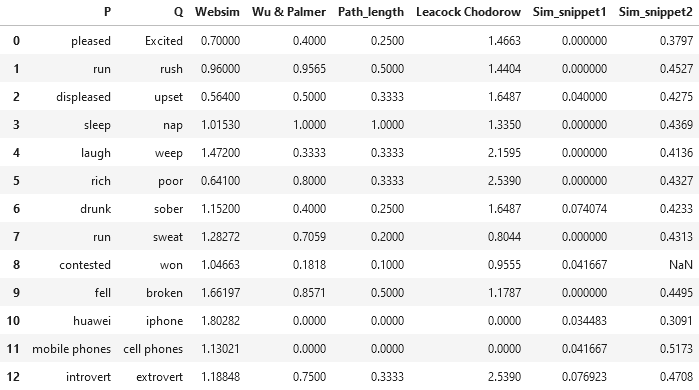
\includegraphics[scale=0.5]{img/table.png}}
\caption{Results for self defined word pairs on similarity methods from chapters~\ref{subsec:webjac} - \ref{subsec:olsim}.}
\label{fig:simtable}
\end{figure}

\newpage
\subsection{Human Judgement Score and Correlations}

As seen in picture~\ref{fig:hjs}, while the results of WUP and PATH differ from the HJS values, LCH comes more closer to latter.

\begin{figure}[h]
\centerline{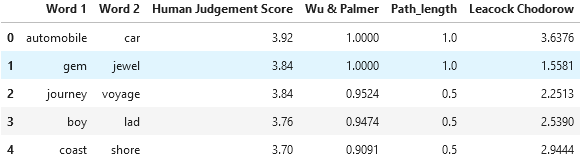
\includegraphics[scale=0.6]{img/hjs.png}}
\caption{Result table of word pairs from MC-28 including WUP, PATH and LCH.}
\label{fig:hjs}
\end{figure}

The correlation data, as resulted according to picture~\ref{fig:wupcorr} between WUP and HJS is very distributed without any noticeable outliers and the correlation between the measurements is very varying. The resulted correlation coefficient of 0.225 shows a lesser correlation rate between both methods.

\begin{figure}[h]
\centerline{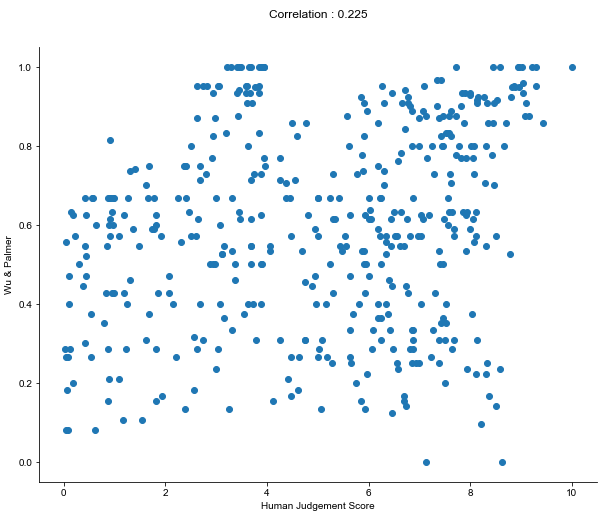
\includegraphics[scale=0.5]{img/wupcorr.png}}
\caption{Correlation between HJS and WUP.}
\label{fig:wupcorr}
\end{figure}

The correlation results beween PATH and HJS, as shown in~\ref{fig:pathcorr}, are noticeably sparsely and linearly distributed in the range between 0 - 0.5 with some positive outliers, and with a correlation coefficient of 0.187 the correlation between those measures are less likely.

\begin{figure}[h]
\centerline{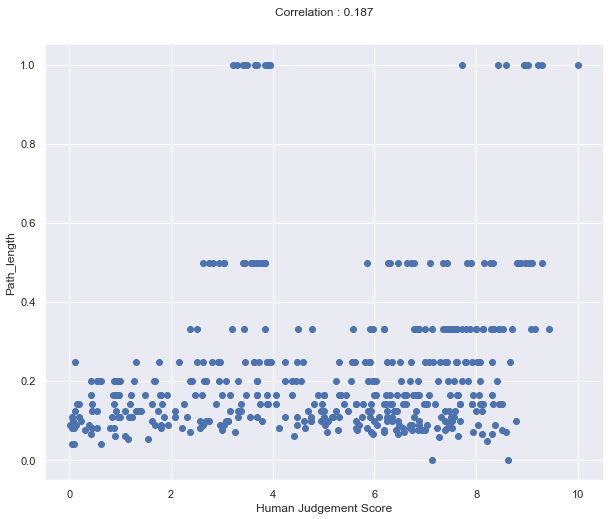
\includegraphics[scale=0.5]{img/pathcorr.png}}
\caption{Correlation between HJS and PATH.}
\label{fig:pathcorr}
\end{figure}

The correlation results beween PATH and HJS, as shown in~\ref{fig:lchcorr}, are again more distributed and with a few outliers in higher values and 0. With a correlation rate of 0.152 however, the correlation coefficient proves a very low correlation rate.

\begin{figure}[h]
\centerline{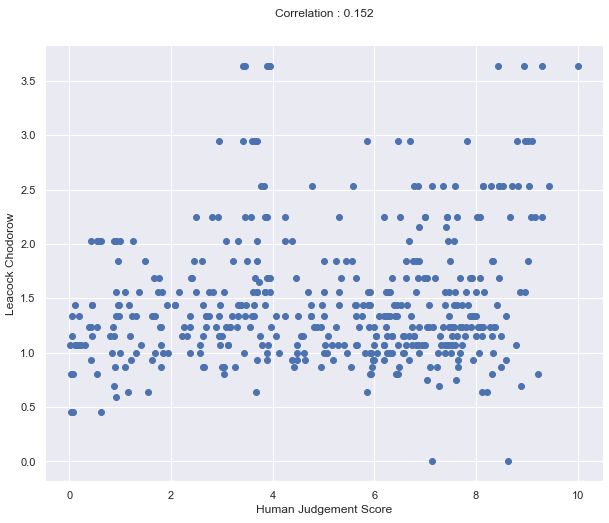
\includegraphics[scale=0.5]{img/lchcorr.png}}
\caption{Correlation between HJS and LCH.}
\label{fig:lchcorr}
\end{figure}

\section{Conclusion}\label{sec:conclusion}

In this project websearch-engine-based dynamic similarity methods were implemented and discussed in comparison to static lexica-based methods.  HJS shows a low correlation rate to the static methods, proving that they are less reliable similarity measurements.. The page-count-based WebSim out-performs the static methods WUP and PATH in most cases and can also measure buzzwords. SnippetSim is not a recommendable measurement method for similarity, as it fails on most word pairs with resulting values of 0. OLSim is more comparable to WUP and PATH and can also use buzzwords. It should be also assumed, that even a high similarity between two pairs can end up in having a bad result if the snippets contain the same contexts but different wordings, as the websearch results are always changing over time. Furthermore, getting the needed websearch results can take time due to the Google Search API'S limit of 100 requests per day, which is the biggest disadvantage of the dynamic methods.

\bibliography{bibtex} 
\bibliographystyle{ieeetran}

\newpage
\begin{appendices}
\section{Source Code of Similarity GUI}\label{sec:append}
\begin{lstlisting}
import tkinter as tk
from tkinter import *
import pandas as pd
#from tkinter.ttk import Progressbar

from implementation import sim, wordnet_sim, sim_snippets1
from implementation import google_snippets, sim_snippets2
#import sys

from pandastable import Table

def get_values():
    word1, word2 = entry1.get(), entry2.get()
    
    if len(word1) ==0:
        tk.messagebox.showinfo('Error', 'Please Enter First Word before finding similarity')
        return None, word2
        
    if len(word2) ==0:
        tk.messagebox.showinfo('Error','Please Enter Second Word before finding similarity')
        word2=None
    
    return word1, word2
    
    
def wordsim(event=None):
    
    word1, word2 = get_values()
    if word1 and word2:
        value = sim(word1, word2, 5)
        tk.messagebox.showinfo('Similarity', 'Word Sim Score : ', round(value, 3))


def net_sim(event=None):
     
    word1, word2 = get_values()
    if word1 and word2:
        a,b,c = wordnet_sim(word1, word2)
        tk.messagebox.showinfo('Wordnet Similarity','WUp: {} , Path: {} , Chod: {}'.
                           format(a,b,c))

def snippet1(event=None):

    word1, word2 = get_values()        
    if word1 and word2:
        snip_p = google_snippets(word1)
        snip_q = google_snippets(word2)
        
        value = sim_snippets1(snip_p, snip_q)
        tk.messagebox.showinfo('Snippet Similarity','Sim SNippet 1 Score: {}'.
                           format(round(value, 2)))
     


def snippet2(event=None):

    word1, word2 = get_values()        
    if word1 and word2:
        snip_p = google_snippets(word1)
        snip_q = google_snippets(word2)
        value = sim_snippets2(snip_p, snip_q)
        tk.messagebox.showinfo('Snippet Similarity','Sim SNippet 2 Score: {}'.
                           format(round(value, 2)))



def exit():
    root.destroy()
    


def gui():
    global root, entry1, entry2
    
    root = tk.Tk()

    lbl=Label(root, text="Simantic Similarity", fg='#37251F', font=("Helvetica", 20))
    lbl.place(x=130, y=30)
    
    lb_e1=Label(root, text="First Word: ", fg='#37251F', font=("Helvetica", 10))
    lb_e1.place(x=90,y=90)
    
    entry1 = tk.Entry(root) 
    entry1.place(x=165, y=90, height=30, width=200)

    lb_e2=Label(root, text="Second Word: ", fg='#37251F', font=("Helvetica", 10))
    lb_e2.place(x=70,y=140)    
    entry2 = tk.Entry(root)
    entry2.place(x=165, y=140, height=30, width=200)
    
    x=172
    button1 = tk.Button(root, text='Web Sim', command=wordsim, fg='white',bg='black', activebackground='#4F2619', height=3,
                  width = 25)
    button1.place(x=x, y=190)
    
    button2 = tk.Button(root, text='Wordnet Sim', command=net_sim, fg='white',bg='black', activebackground='#4F2619', height=3,
                  width = 25)
    button2.place(x=x, y=260)
    
    button3 = tk.Button(root, text='Sim Snippet 1', command=snippet1, fg='white',bg='black', activebackground='#4F2619', height=3,
                  width = 25)
    button3.place(x=x, y=330)
    
    button4 = tk.Button(root, text='Sim Snippet 2', command=snippet2, fg='white',bg='black', activebackground='#4F2619', height=3,
                  width = 25)
    button4.place(x=x, y=400)

    button5 = tk.Button(root, text='Exit', command=exit, fg='white',bg='black', activebackground='#4F2619', height=3,
                  width = 25)
    button5.place(x=x, y=470)
    
    root.title('Application')
    root.geometry("500x650+300+20")
    root.mainloop()


if __name__ == '__main__':

    gui()
\end{lstlisting}
\end{appendices}

\end{document}
